
\let\negmedspace\undefined
\let\negthickspace\undefined
\documentclass[journal]{IEEEtran}
\usepackage[a5paper, margin=10mm, onecolumn]{geometry}
%\usepackage{lmodern} % Ensure lmodern is loaded for pdflatex
\usepackage{tfrupee} % Include tfrupee package
\setlength{\headheight}{1cm} % Set the height of the header box
\setlength{\headsep}{0mm}     % Set the distance between the header box and the top of the text
\usepackage{gvv-book}
\usepackage{gvv}
\usepackage{cite}
\usepackage{amsmath,amssymb,amsfonts,amsthm}
\usepackage{algorithmic}
\usepackage{graphicx}
\usepackage{textcomp}
\usepackage{xcolor}
\usepackage{txfonts}
\usepackage{listings}
\usepackage{enumitem}
\usepackage{mathtools}
\usepackage{gensymb}
\usepackage{comment}
\usepackage[breaklinks=true]{hyperref}
\usepackage{tkz-euclide} 
\usepackage{listings}
% \usepackage{gvv}                                        
\def\inputGnumericTable{}                                 
\usepackage[latin1]{inputenc}                                
\usepackage{color}                                            
\usepackage{array}                                            
\usepackage{longtable}                                       
\usepackage{calc}                                             
\usepackage{multirow}                                         
\usepackage{hhline}                                           
\usepackage{ifthen}                                           
\usepackage{lscape}
\renewcommand{\thefigure}{\theenumi}
\renewcommand{\thetable}{\theenumi}
\setlength{\intextsep}{10pt} % Space between text and floats
\numberwithin{equation}{enumi}
\numberwithin{figure}{enumi}
\renewcommand{\thetable}{\theenumi}
\begin{document}
\bibliographystyle{IEEEtran}
\title{12.9.7.3}
\author{EE24BTECH11041 - Mohit}
% \maketitle
% \newpage
% \bigskip
{\let\newpage\relax\maketitle}
\begin{enumerate}
	\item From the differential equation representing the family of curves given by $\brak{x-a}^2 + y^2 = a^2$, where $a$ is an arbitrary conatant.
\textbf{Solution:-}\\
\begin{enumerate}
\item Simplyfying the equation to,
\begin{align}
x^2-2ax+2y^2=0\\
a = \frac{x^2+2y^2}{2x}
\end{align}
\item Differtiating the Equation 1 with respect to x
\begin{align}
	2x-2a+4y\frac{dy}{dx}=0
\end{align}
\item Substituing 2nd equation in 3rd equation
\begin{align}
	\frac{x^2-2y}{x} + 4y\frac{dy}{dx} = 0	
\end{align}



The given differential equation is:

\begin{align}
\frac{x^2 - y}{x} + 4y \frac{dy}{dx} = 0
\end{align}


\item \textbf{Simplify the equation:}

Rewrite the equation:

\begin{align}
\frac{x^2}{x} - \frac{2y}{x} + 4y \frac{dy}{dx} &= 0 \\
x - \frac{2y}{x} + 4y \frac{dy}{dx} &= 0 \\
x + 4y \frac{dy}{dx} &= \frac{2y}{x}.
\end{align}

Rearranging gives:

\begin{align}
4y \frac{dy}{dx} &= \frac{2y}{x} - x.
\end{align}

\item \textbf{Separate the variables:}

Divide through by $y$ (assuming \(y \neq 0\)):

\begin{align}
\frac{dy}{dx} &= \frac{1}{4}\brak{\frac{2}{x} - \frac{x}{y}}
\end{align}



\item \textbf{CODING LOGIC:} The solution for the differential equation can be graphically solved using coding by using below logic :

\begin{align} 
	x_0 &= 0.001 \\ 
	y_0 &= 0.031 \\
	h&=0.01 \\
	y_{n+1} &= y_{n} + h\cdot\brak{\frac{dy}{dx}} \\ 
	y_{n+1} &= y_{n} + h\cdot\brak{\frac{1}{4}\brak{\frac{2}{x} - \frac{x}{y}}} \\ 
	x_{n+1} &= x_{n} + h 
\end{align}

Solving Question for a=1


\begin{figure}[h!]
   \centering
   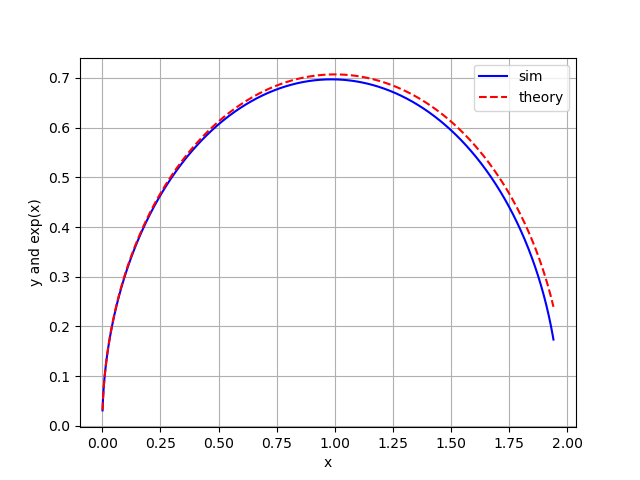
\includegraphics[width=0.7\linewidth]{figs/Figure_1.png}
\end{figure}
\end{enumerate}
\end{enumerate}
\end{document}
